\chapter{How to Use the utdiss2 Package}
\index{How to Use the utdiss2 Package%
@\emph{How to Use the utdiss2 Package}}%

\section{WebCore: Web-Specific Mobile Processor Architecture}
\label{sec:arch}

Domain-specific specialized architecture has long been deemed as extremely high-performance and energy-efficient because it aggregates hundreds of operations in a few instructions and, therefore, reduces major sources of inefficiencies in general-purpose CPUs~\cite{h264, soda, anysp}. The key challenge of applying architectural specialization to Web computing is how to \textit{retain general-purpose programmability}. The general-purpose programmability is a particular necessity for Web technologies because they involve large pieces of software that are written in a combination of different general-purpose programming languages. For example, Google's Chrome Web browser is developed in 29 languages with over 17 million lines of code~\cite{chromeloc}. Recent work has demonstrated the importance and feasibility of balancing general-purpose programmability and specialization in various data computation domains (e.g., H.264 encoding~\cite{h264}, convolution~\cite{ce}).

Following the same architecture design philosophy of balancing general-purpose programmability and domain-specific specialization, I propose the \webcore, a general-purpose CPU customized and specialized for Web technologies. \webcore's design starts from existing mobile CPUs, and thus retains the general-purpose programmability. It achieves performance and energy improvement by combining customization and specialization techniques. In the rest of this section, I describe the customization and specialization process in \Sect{sec:arch:customization} and \Sect{sec:arch:specialization}, respectively. \Sect{sec:arch:related} discusses prior work on hardware support for mobile Web.

\subsection{Customizing General-Purpose Cores}
\label{sec:arch:customization}

\webcore design is based on general-purpose CPUs to best retain the general-purpose programmability. However, existing general-purpose processors may not be an ideal baseline for \webcore, because they are not uniquely tuned for Web applications. \webcore customizes current designs by exploring a vast design space to properly size key microarchitecture parameters.

I derive two major conclusions through the customization process. First, out-of-order designs provide more flexibility for energy versus performance trade-offs than in-order designs. Second, a customized out-of-order design configuration still contains two sources of inefficiency---instruction delivery and data feeding---that need to be further mitigated.

\paragraph{Design Space Exploration (DSE)} We mine through the top 10,000 websites as ranked by Alexa~\cite{alexa} and leverage the principal component analysis (PCA) to select the 12 most representative websites. All except one happen to rank among Alexa's top 25 websites. We consider both mobile and desktop versions of the 12 websites because tablets typically load the desktop version of webpages. In total, we study 24 distinct webpages.

We consider various tunable microarchitectural parameters such as issue width, instruction/data cache sizes. We vary the values of functionally related parameters (e.g., issue width and the number of functional units) together to avoid reaching an entirely unbalanced design~\cite{ilp2}. We also do not consider single-issue out-of-order processors, which are known to be energy inefficient~\cite{marginal}. In total, we consider over 3~billion design points.

It is not feasible to simulate all of the design points simply due to time constraints. Therefore, we leverage regression modeling techniques~\cite{RMS} to predict the performance and power consumption of various design points in the space. Such effort has been used successfully in the past for architecture design-space exploration~\cite{dse, comt}. We construct performance and power models for in-order and out-of-order designs separately. Overall, the out-of-order models' error rates are below 6.0\%. The in-order performance and power models' errors are within 5\% and 2\%, respectively. The in-order models are more accurate because of their simpler design.

\begin{figure}[t]
\centering
  \begin{minipage}[b]{0.3\columnwidth}
  	\centering
  	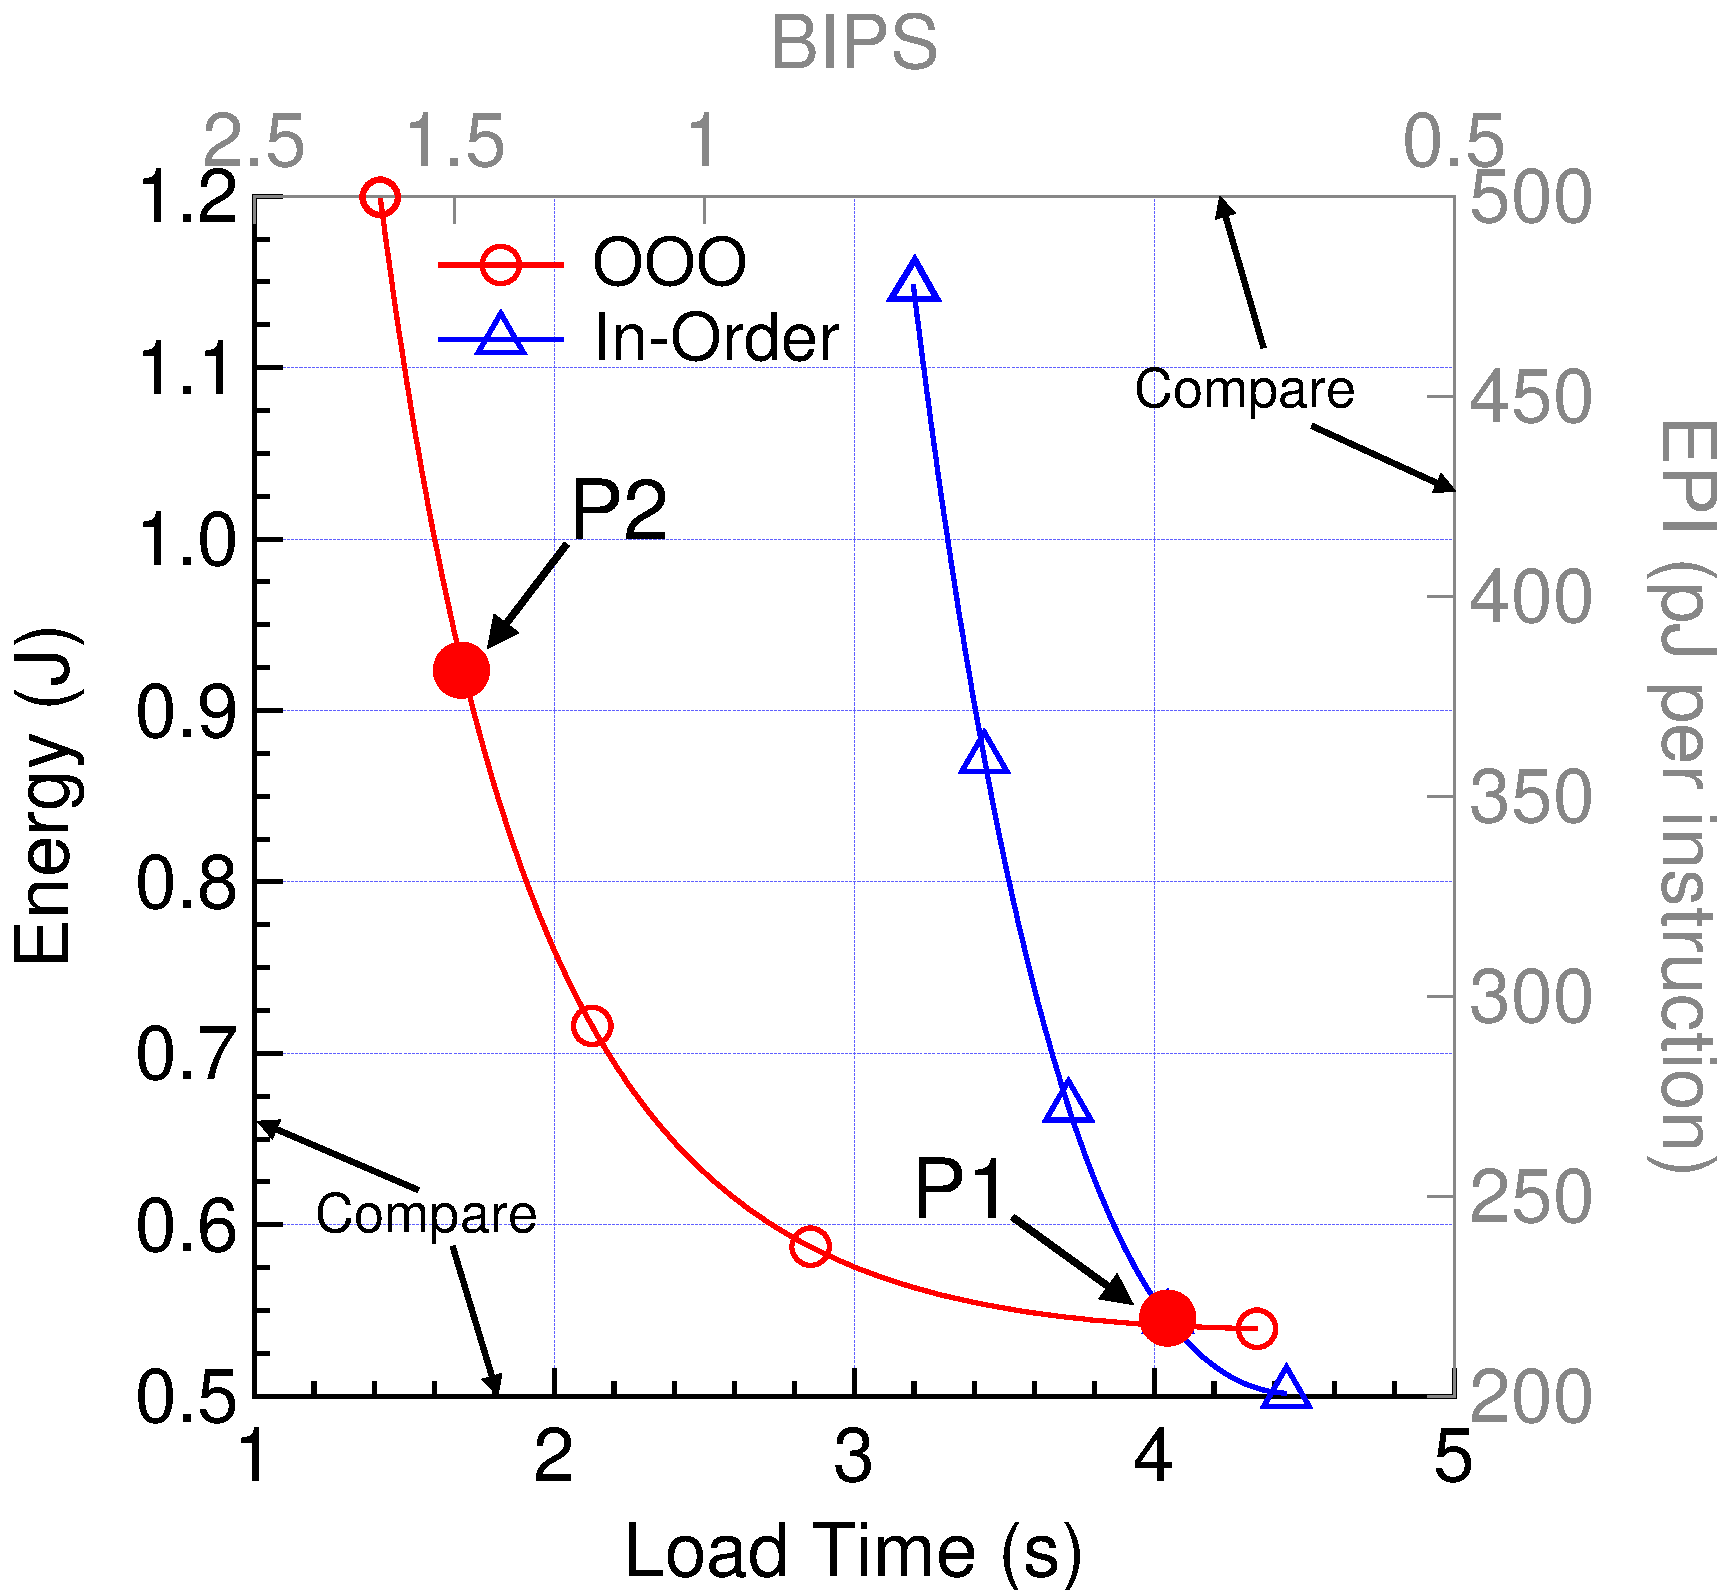
\includegraphics[trim=0 0 0 0, clip, width=\columnwidth]{ivso}
  	\caption{In-order versus out-of-order Pareto optimal frontiers.}
  	\label{fig:ivso}
  \end{minipage}
  \hspace*{10pt}
  \begin{minipage}[b]{0.3\columnwidth}
  	\centering
  	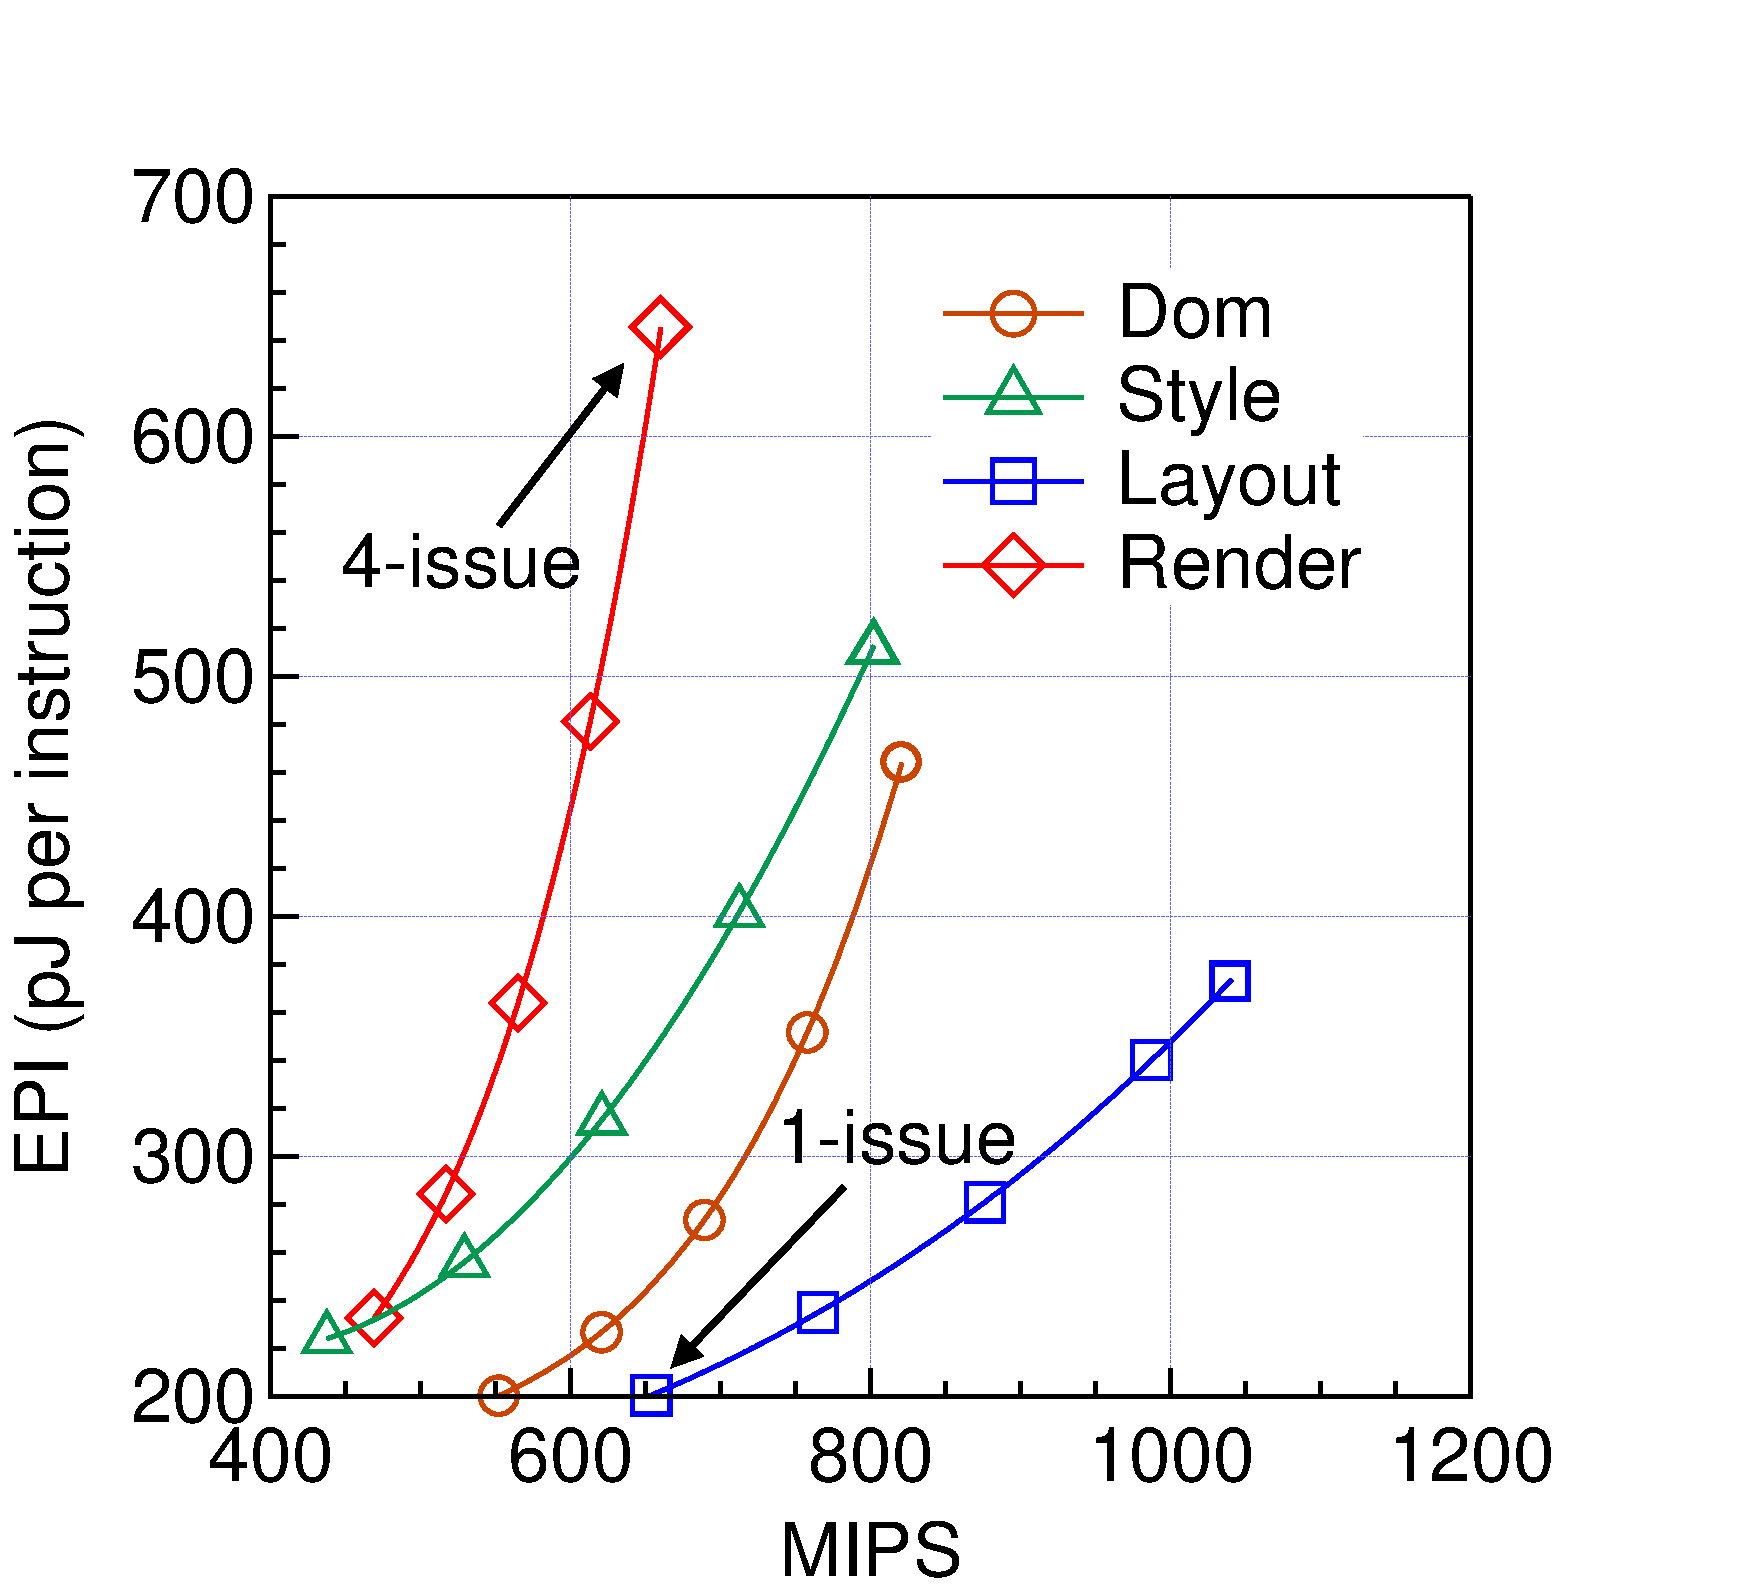
\includegraphics[trim=0 0 0 0, clip, width=\columnwidth]{pareto_io}
  	\caption{In-order Pareto optimal frontier for each kernel.}
  	\label{fig:pareto_io}
  \end{minipage}
  \hspace*{10pt}
  \begin{minipage}[b]{0.3\columnwidth}
  	\centering
  	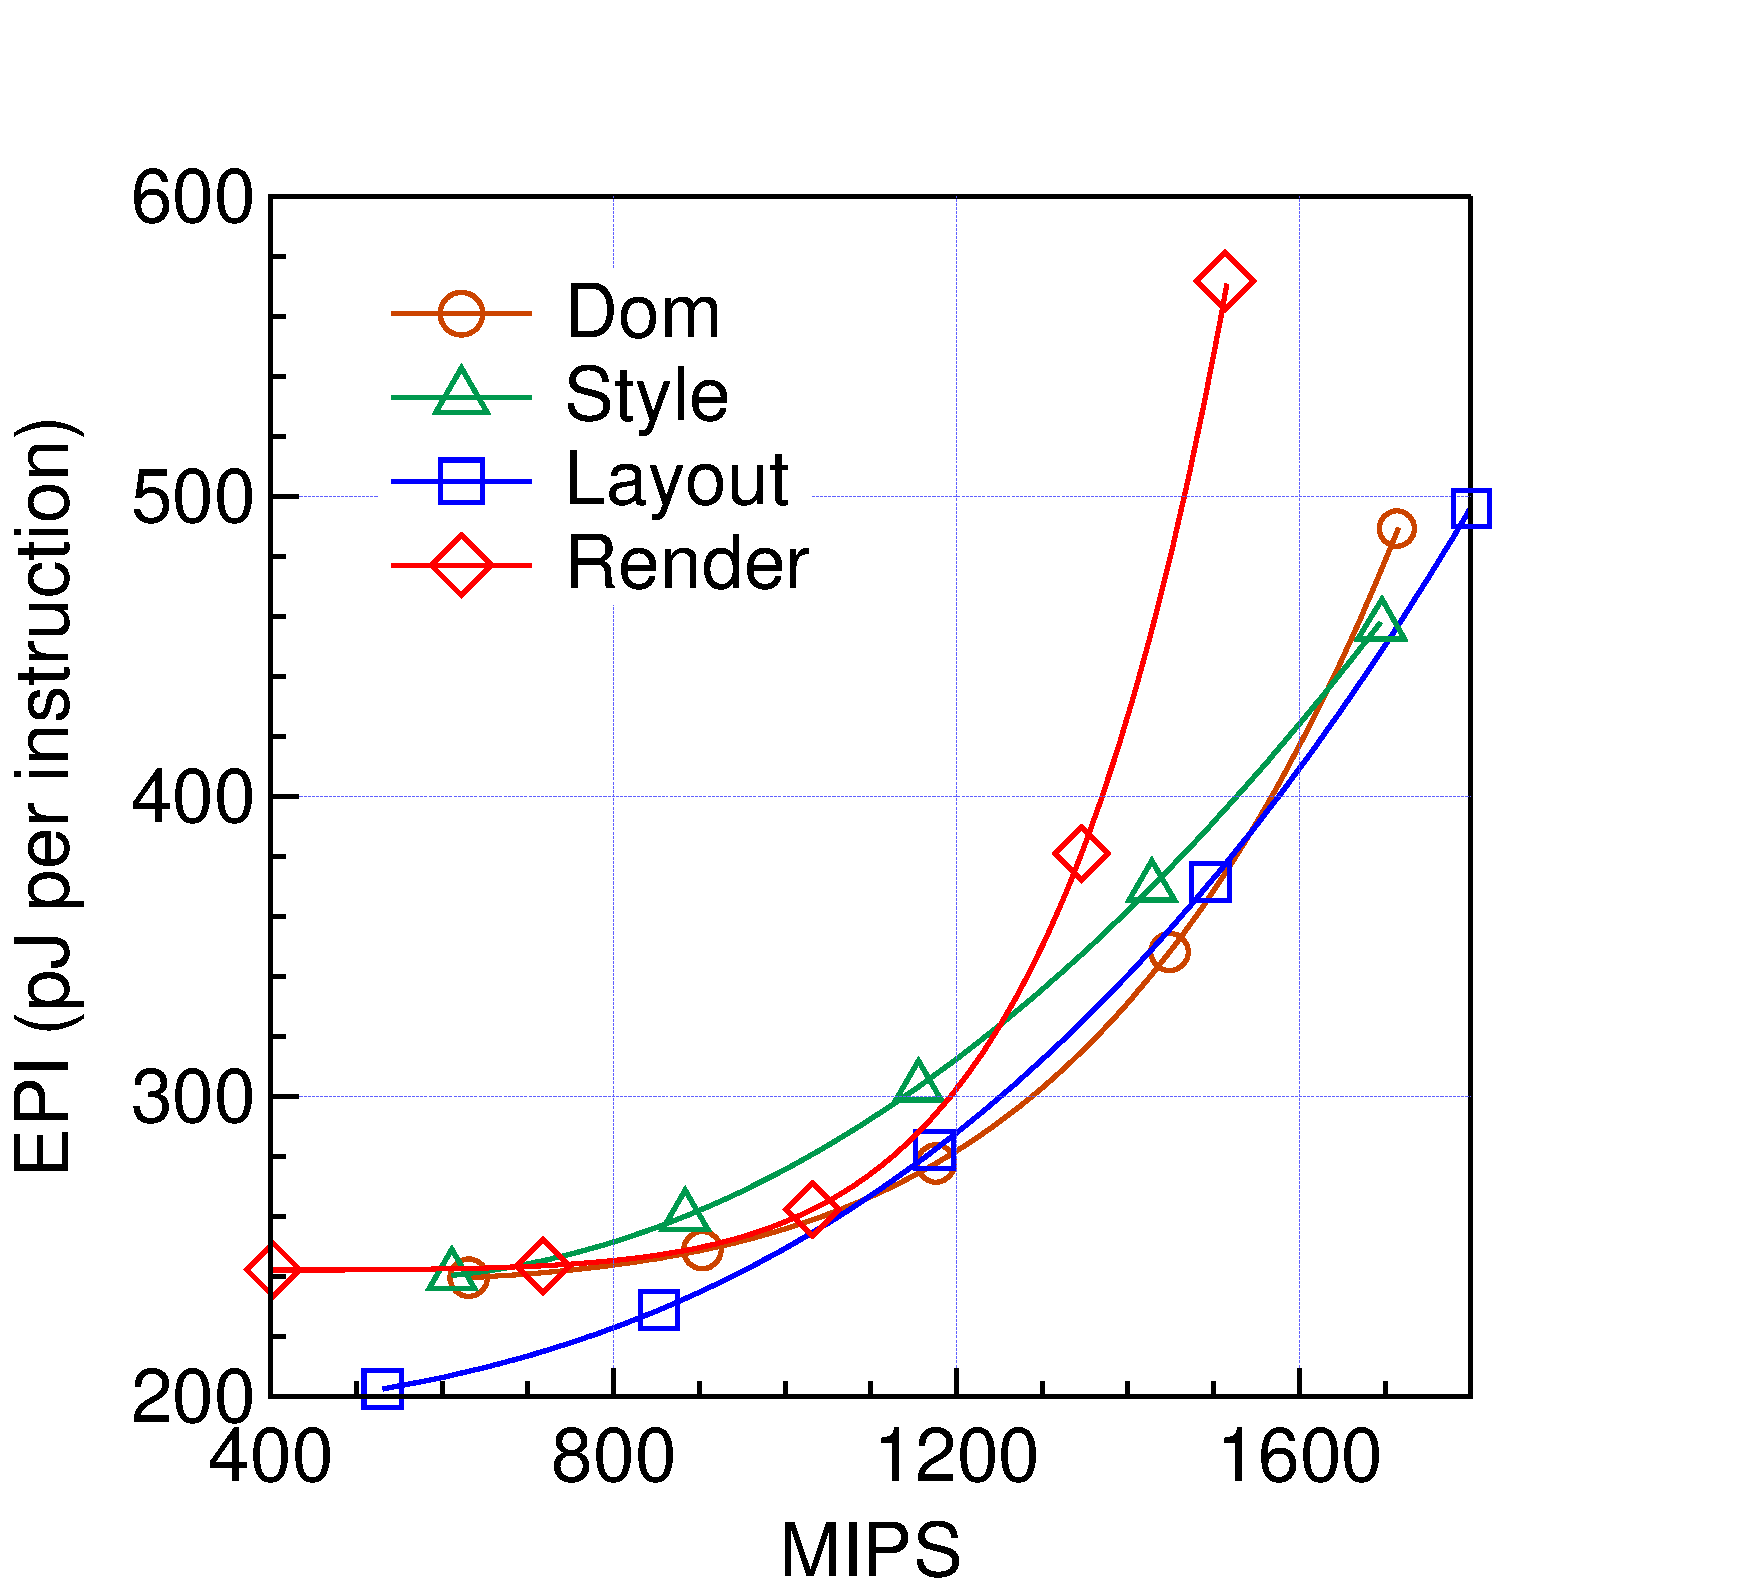
\includegraphics[trim=0 0 0 0, clip, width=\columnwidth]{pareto_ooo}
  	\caption{Out-of-order Pareto optimal frontier for each kernel.}
  	\label{fig:pareto_ooo}
  \end{minipage}
\end{figure}

\paragraph{Core Choice} Design space exploration helps customization at the ``macro-architecture'' level, i.e., determining between in-order and out-of-order designs. We understand the difference between in-order and out-of-order design space by examining their Pareto optimal frontiers. Design points on a Pareto optimal frontier reflect different optimal design decisions given specific performance/energy targets. \Fig{fig:ivso} shows the Pareto optimal frontiers of the in-order and out-of-order design space. We observe that the in-order design space has a narrow performance range of 1~second, whereas the out-of-order space covers a 4~second performance range. The performance range contrast indicates that out-of-order designs can more flexibly balance performance with energy and, therefore, are better design baselines for mobile Web applications.

To understand the difference behind the in-order versus out-of-order designs, we study the kernel behaviors in Web applications. There are four important computation kernels in executing a Web application: i.e.,~\textit{Dom}, \textit{Style}, \textit{Layout}, and \textit{Render}. They contribute to about 75\% of the webpage load time and energy consumption.~\Fig{fig:pareto_io} and~\Fig{fig:pareto_ooo} show the Pareto optimal frontiers of the in-order and out-of-order design space for each kernel. We find that the kernel variance in the in-order designs is more pronounced than in the out-of-order designs. As we push toward more performance in the in-order design space, some kernels stop scaling gracefully on the energy-versus-delay curve, and eventually become a performance bottleneck. Overall, in-order designs have low marginal performance value with high marginal energy cost~\cite{marginal}. In contrast, out-of-order cores can cover the variances across the different kernels through complex execution logic and, therefore, provide wider performance and energy trade-off range.

\begin{table}[t]
\large
\centering
\captionsetup{width=.6\columnwidth}
\caption{\small Microarchitecture configurations for P1 and P2 in
\Fig{fig:ivso}. They represent different energy-delay trade-offs. For comparison
purpose, we also show the parameters for ARM Cortex-A15, whose information is
gather from measurements using the 7-Zip LZMA Benchmark~\cite{7cpu-a15} and
ARM's public presentation~\cite{a15-slide}.}
\renewcommand*{\arraystretch}{1.2}
\renewcommand*{\tabcolsep}{10pt}
\resizebox{.6\columnwidth}{!}
{
	\begin{tabular}{l l l l}
	\toprule[0.15em]
        ~      & \bigstrut\textbf{P1} & \bigstrut\textbf{P2} & \bigstrut\textbf{Cortex-A15}\\
	\midrule[0.05em]
        Issue width						&	1		&	3	&	3	\\
        \# Functional units				&	2		&	3	&	8	\\
        Load queue size (\# entries)		&	4		&	16	&	16	\\
        Store queue size (\# entries)	&	4		&	16	&	16	\\
        BTB size (\# entries)   &       1024    &       128 &   64       \\
        ROB size (\# entries)			&	128		&	128	&	40+	\\
        \# Physical registers			&	128		&	128	&	?	\\
        L1 I-cache size (KB)				&	64		&	128	&	32	\\
        L1 I-cache delay (cycles)		&	1		&	2	&	?	\\
        L1 D-cache size (KB)				&	8		&	64	&	32	\\
        L1 D-cache delay (cycles)		&	1		&	1	&	4	\\
        L2 cache size (KB)				&	256&	1024	&	512\textasciitilde4096	\\
        L2 cache delay (cycles)			&	16		&	16	&	21	\\
	\bottomrule[0.15em]
    \end{tabular}
}
\label{tab:dse:ednp}
\end{table}

\paragraph{Sources of Inefficiency} DSE also helps customization at the microarchitecture level. We examine microarchitectural parameters of two out-of-order Pareto optimal designs: P1 and P2 in \Fig{fig:ivso}. They represent designs optimized for different performance and energy targets. P1 is optimized for minimal energy consumption in the out-of-order space. P2 is a high-performance design with a performance of 1500 MIPS (million instructions per second). \Tbl{tab:dse:ednp} summarizes the microarchitecture configurations of the two designs. For comparison purposes, it also lists the same parameters for ARM Cortex-A15, which represents today's high-end mobile CPU.

By comparing P1 and P2 with Cortex-A15, we find two major sources of inefficiencies in general-purpose processors: instruction delivery and data feeding. First, current mobile processors have a small L1 instruction cache that is typically 32~KB in size. However, the two Pareto optimal designs require a 64~KB to 128~KB instruction cache to alleviate the pressure on instruction delivery in mobile Web applications. The pathological front-end behavior mainly stems from the large instruction footprint and the prevalence of the irregular control flow path~\cite{bbench}.

Second, the high-performance design P2 also necessitate a 64~KB data cache, doubling the typical L1 data cache size in current mobile CPUs. The need for a large data cache mainly stems from the large working set size on principal data structures (e.g., the DOM tree) during webpage processing. For example, profiling results show that the average data reuse distance for DOM tree accesses is 4~KB (excluding other memory operations interleaved with DOM accesses). The large data cache leads to excessive energy consumption and needs to be optimized.

\subsection{Specializing the Customized Cores}
\label{sec:arch:specialization}

Unusual design parameters in a customized processor tuned for the mobile Web workload indicate that instruction delivery and data feeding are critical to guarantee high performance while still being energy efficient. I propose a specialized functional unit that mitigates the two bottlenecks. The new hardware structure is accessed via a set of high-level language APIs implemented as a runtime library to maintain the general-purpose programmability.

\paragraph{Style Resolution Unit} The \textit{Style} kernel is an important computation kernel in a Web browser~\cite{webcore}. It takes about one-third of the total execution time and energy consumption of webpage loading. Therefore, optimizing the \textit{Style} kernel would provide the most overall benefits. In order to mitigate the instruction delivery and data communication overhead of the~\textit{Style} kernel, I propose a hardware functional unit called the~\textit{Style Resolution Unit} (SRU). The SRU design is based on the observation that the \textit{Style} kernel has abundant fine-grained parallelism that is hidden in a software implementation but can be captured by a dedicated hardware structure. To exploit the inherent fine-grained parallelism, the SRU employs a multi-lane parallel architecture, which greatly reduces the instruction delivery overhead. To reduce the data feeding pressure, the SRU is tightly coupled with a small scratchpad memory that brings operands closer to the SRU.

\begin{figure}[t]
  \centering
  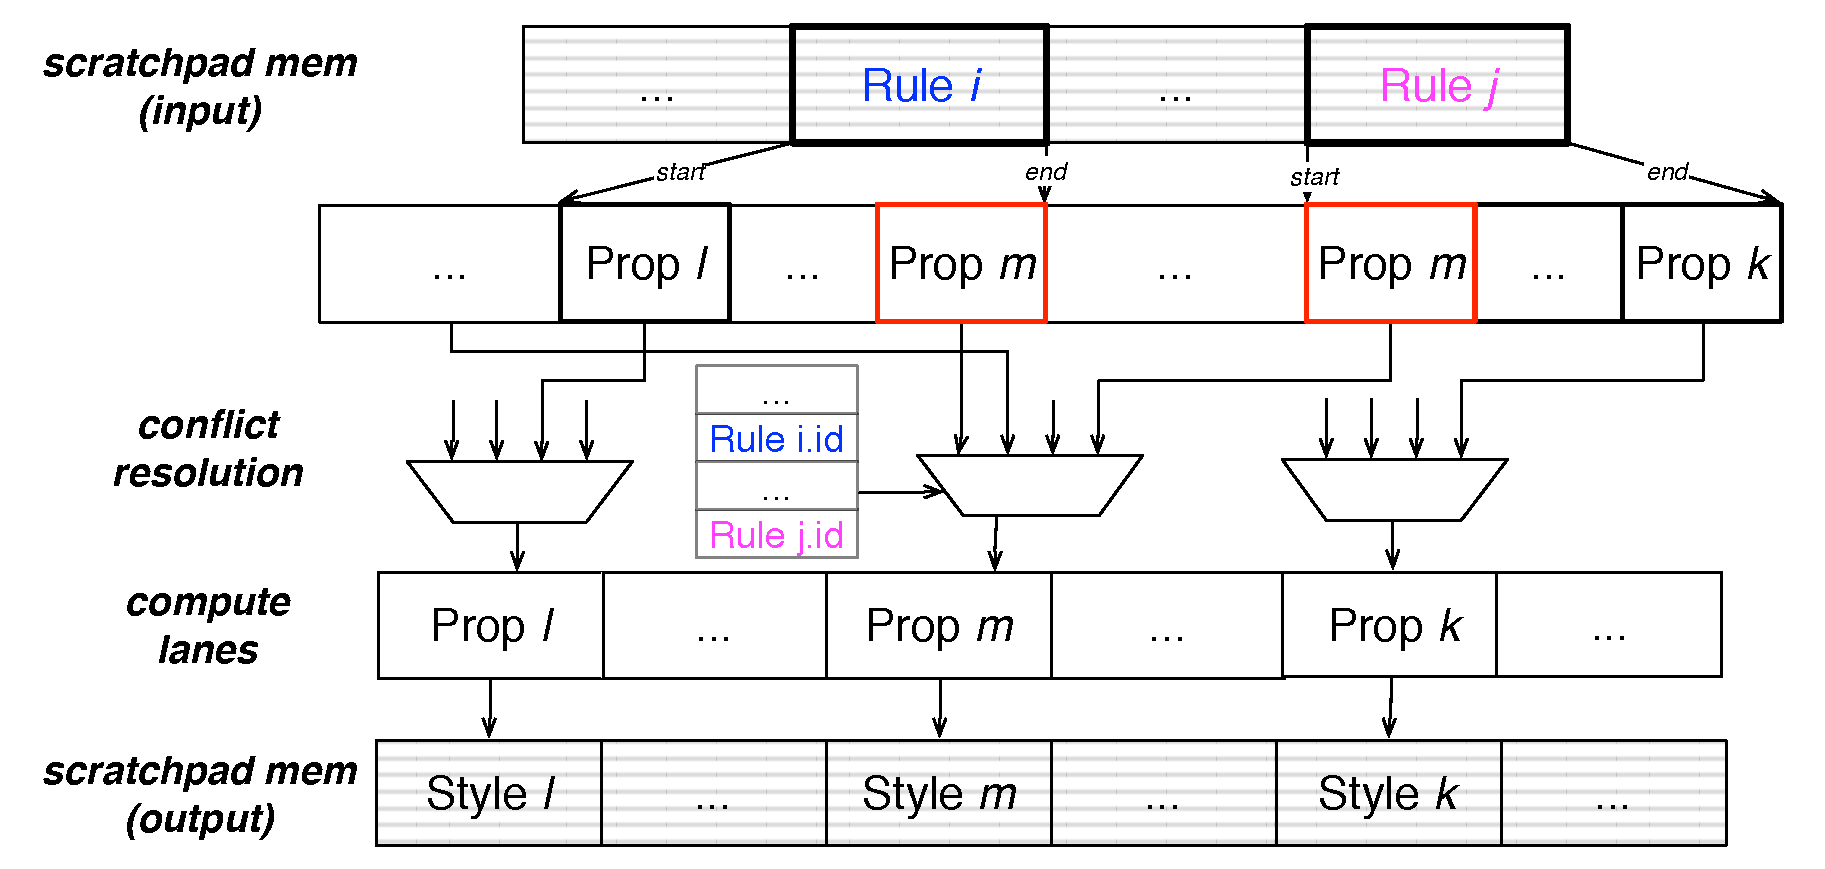
\includegraphics[trim=0 0 0 0, width=.7\columnwidth]{sru}
  \caption{\small{SRU coupled with scratchpad memories.}}
  \label{fig:sru}
\end{figure}

The \textit{Style} kernel takes a set of input CSS rules, and applies the rules in certain cascading order~\cite{cascading} to calculate a final value of each CSS property (e.g., the exact RGB values for the \texttt{color} property, or the number of pixels for the \texttt{width} property). These values are stored back to a data structure called render tree for further processing by other kernels.

The key observation we make from the \textit{Style} kernel algorithm is that there are two types of inherent parallelism: ``rule-level parallelism'' (RLP) and ``property-level parallelism'' (PLP). Improving the performance and energy consumption of the~\textit{Style} kernel requires us to exploit both forms of parallelism. RLP comes from the following observation. In the sequential algorithm, each rule must be iterated from the lowest priority to the highest following the cascading order~\cite{cascading}, so that values from higher-priority rules can override values from lower-priority rules. However, we could speculatively apply rules with different priorities in parallel, and simply select the correct value according to the rule priorities in the end. PLP follows RLP. Each rule contains value information of multiple CSS properties. Calculating values for all the properties contained within a rule is independent of each other, and can be executed in parallel.

We propose Style Resolution Unit (SRU) as a parallel hardware unit to exploit both RLP and PLP. The SRU aggregates enough computations to reduce control-flow divergences and increase arithmetic intensity. It is accompanied by scratchpad memory that reduces the overhead of data communication for both input and output. \Fig{fig:sru} shows the structure of the SRU with scratchpad memory. SRU is a SIMD-like structure with multiple compute lanes, with each lane calculating the final value of one CSS property. Assume Rule~$i$ and Rule~$j$ are two rules from the input that are residing in the scratchpad memory. Rule~$i$ has higher priority than Rule~$j$. Prop~$l$ and Prop~$m$ are two properties in Rule~$i$. Similarly, Rule~$j$ has properties Prop $k$ and Prop $m$. Prop~$l$ and Prop~$k$ can be executed in parallel using different SRU lanes because they do not conflict with each other. However, Prop~$m$ is present in both rules, and as such it causes an SRU lane conflict, in which case the MUX selects the property from Rule~$i$ because it has a higher priority. The compute lanes then write the final values back to the output scratchpad memory.

\paragraph{Implementation Details} A hardware implementation can have only a fixed amount of resources. Therefore, the number of SRU lanes and the size of the scratchpad memory is limited. We profile the webpages to determine the appropriate amount of resource allocation. Profiling indicates that 90\% of the time, the RLP is below or equal to 4. Therefore, our design's scratchpad memory only stores up to four styles. Similarly, 32 hot CSS properties cover about 70\% of the commonly used properties. Thus, we implement a 32-wide SRU where each lane handles one hot CSS property.

Due to these considerations, the scratchpad memories are each 1~KB in size. Under Synposys 28~nm toolchain, the total area overhead of SRU is about 0.59 mm$^2$, negligible compared to typical mobile SoC size (e.g., Samsung's Exynos 5410 SoC has a total die area size of 122~mm\textsuperscript{2}~\cite{exynox5410diesize}). The SRU logic introduces 70~mW total power, which is insignificant compared to power consumption in a typical mobile CPU (e.g., about 1~W on a single core Cortex-A15). The scratchpad memory can be accessed in one cycle, which is the same as the fastest L1 cache latency in our design space. The SRU logic latency is about 16 cycles under 1.6~GHz.

\paragraph{Software Support and Programmability} The SRU can be accessed via an instruction extension to the general-purpose ISA. In order to abstract the low-level details away from application developers, we provide an library API in high-level languages. Application developers use the API without knowing the existence of the SRU. It is important to notice that these software APIs are used by Web browser rendering engine developers rather than high-level Web application developers. SRU does not affect the programming interface of Web application developers and, therefore, has no impact on the Web application development productivity.

Programmers trigger the style resolution task by issuing a~\texttt{Style\_Apply(Id, Rules)} API, in which \texttt{Id} represents a DOM tree node ID and \texttt{Rules} represents matched CSS rules produced by the matching phase. One key task of this API implementation is to examine all the CSS properties of a particular DOM node because not all the CSS properties are implemented in the SRU. For properties that can be offloaded to the SRU, the API implementation loads related data into the SRU's scratchpad memory. For those ``unaccelerated'' properties, the runtime creates the necessary compensation code. Specifically, we propose relying on the existing software implementation as a fail-safe fallback mechanism. Once the style resolution results are generated, the results can be copied out to the output scratchpad memory.

\subsection{Related Work}
\label{sec:arch:related}

Similar to \webcore, SiChrome~\cite{SiChrome} performs aggressive specializations that map much of the Chrome browser into silicon. The key difference is that \webcore starts from a (well-optimized) general-purpose baseline and thus retains general-purpose programmability while still being energy-efficient. In addition, SiChrome evaluates energy-efficiency using the EDP metric while our Pareto optimal analysis provides a more generic optimization view than EDP.

EFetch~\cite{efetch} and ESP~\cite{esp} also propose specialized hardware structures on top of general-purpose cores to improve the performance and energy-efficiency of Web applications. They view a Web application execution as a sequence of events. As a result, the proposed specialized hardware primarily targets the inefficiencies associated with the event-driven execution model. \webcore views a Web application execution as a mix of different kernels. As such, the proposed specialization technique targets individual kernels. Both views are complementary in that per-event execution can benefit from kernel-level improvement that \webcore provides and vice versa.

%\subsection{Preliminary Results}
%\label{sec:arch:res}
%
%\begin{figure}[t]
%\centering
%  \begin{minipage}[b]{0.3\columnwidth}
%    \centering
%    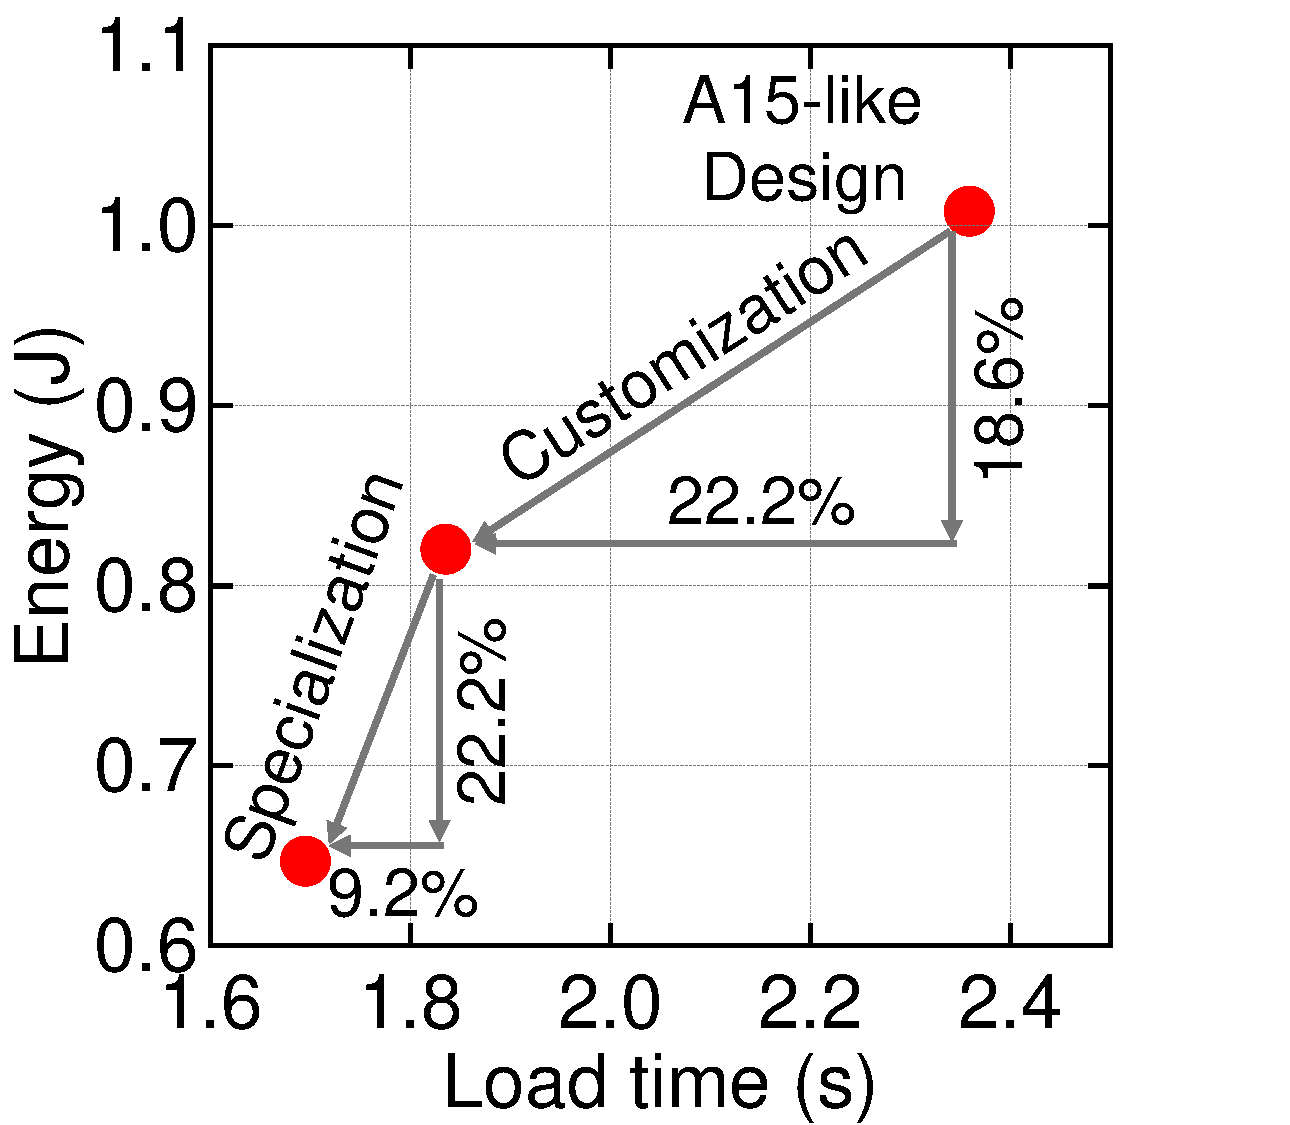
\includegraphics[trim=0 00 0 0, clip, width=\columnwidth]{results}
%    \caption{\small{Energy consumption and performance improvement of customization and specialization. The baseline is an ARM Cortex-A15 like mobile CPU.}}
%    \label{fig:results}
%  \end{minipage}
%  \hspace*{25pt}
%  \begin{minipage}[b]{0.3\columnwidth}
%    \centering
%    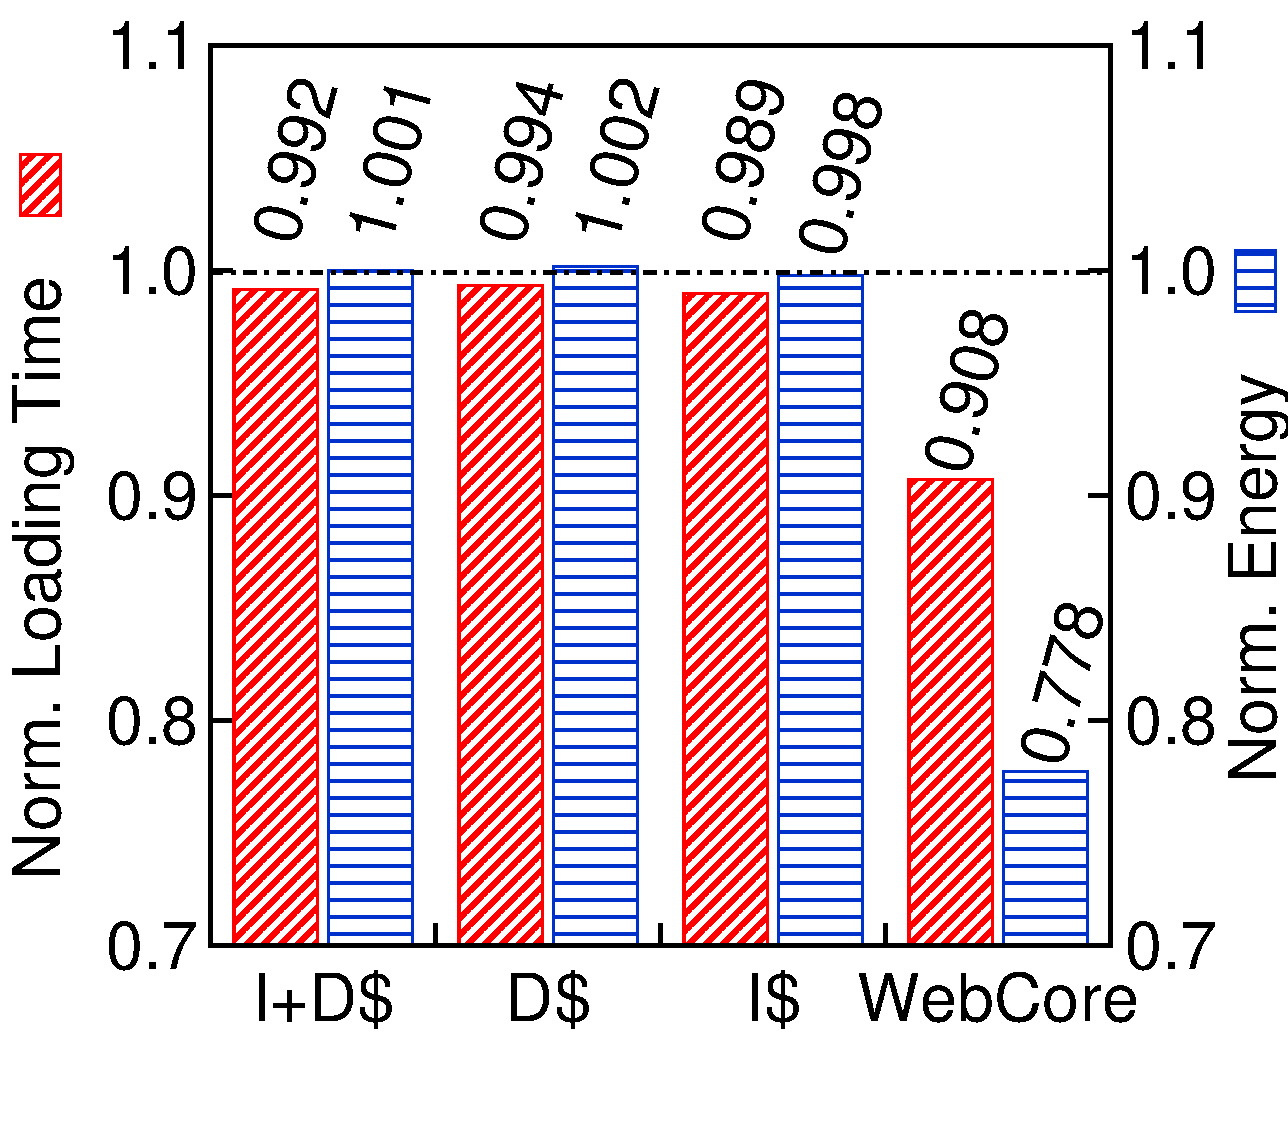
\includegraphics[trim=0 0 0 0, clip, width=\columnwidth]{compare-other}
%    \caption{\small{Comparison between specialization techniques in WebCore against using the additional area to increase instruction and/or data cache sizes.}}
%    \label{fig:compare-other}
%  \end{minipage}
%\end{figure}
%
%We implement the \webcore specializations in Verilog and synthesize our design in 28~nm technology using the Synposys toolchain. We use CACTI v5.3~\cite{cacti} to estimate the memory structures' overhead. In total, the area overhead is about 0.59~mm\textsuperscript{2}, insignificant compared to a typical mobile CPU size~\cite{exynox5410coresize}. The total power overhead is about 80~mW, insignificant compared to the total power consumption at about 1~W. The SRU logic latency is about 16 cycles under 1.6~GHz.
%
%We use~\Fig{fig:results} to illustrate the effectiveness of \webcore. We start from an ARM Cortex-A15 like processor, and progressively apply customization and specialization. Customization alone leads to 22.2\% performance improvement and 18.6\% energy saving. Specializations gain an additional 9.2\% performance improvement and 22.2\% energy saving. The accelerated~\textit{Style} kernel achieves up to 10X speedup. Overall, \webcore improves performance by 29.2\% and saves 47.0\% energy.
%
%To further to justify the effort needed for the specialization techniques in the \webcore, we also compare \webcore with conventional strategies that simply scale up the microarchitecture structures under the same area overhead of \webcore. Specifically, we compare with designs that improve the I-cache and D-cache sizes because instruction delivery and data feeding are the two major bottlenecks. \Fig{fig:compare-other} compares \webcore with designs that increase the I-cache size by 24~KB (I\$), the D-cache size by 24~KB (I\$), and both caches by 12~KB (I+D\$). The figure normalizes the webpage loading time and energy consumption to \webcore without any specializations. We observe that simply improving the cache sizes in general-purpose cores achieves only negligible performance improvement (<1\%) with a slightly higher energy consumption. However, \webcore specializations provide significantly better performance and energy improvements.


%%%%%%%%%%%%%%%%%%%%%%%%%%%%%%
%\paragraph{Browser Engine Cache} The DOM tree and Render tree are the two most
%important data structures because they are shared across different kernels. I
%propose the~\textit{Browser Engine Cache} (BEC) to reducing the energy of
%accessing these data structures. BEC is motivated by the unique access patterns
%to the DOM tree and render tree. They have strong locality that can benefit from
%a small and energy-efficient L0 cache-like memory, rather than the large
%power-hungry traditional caches
%
%The BEC consists of a DOM cache and a Render cache. We use the DOM to explain
%our locality observation. \Fig{fig:con-reuse} shows the cumulative distribution
%of DOM tree node reuse. Each~($x, y$) point corresponds to a portion of DOM tree
%nodes~($y$) that are consecutively reused at least a certain number of
%times~($x$). About 90\% of the DOM tree nodes are consecutively reused at least
%three times, indicating strong data locality. The strong locality suggests that
%a very small cache could achieve the same hit rate as a regular cache, but with
%much lower power.
%
%\begin{figure}[t]
%\centering
%  \begin{minipage}[b]{0.3\columnwidth}
%    \centering
%    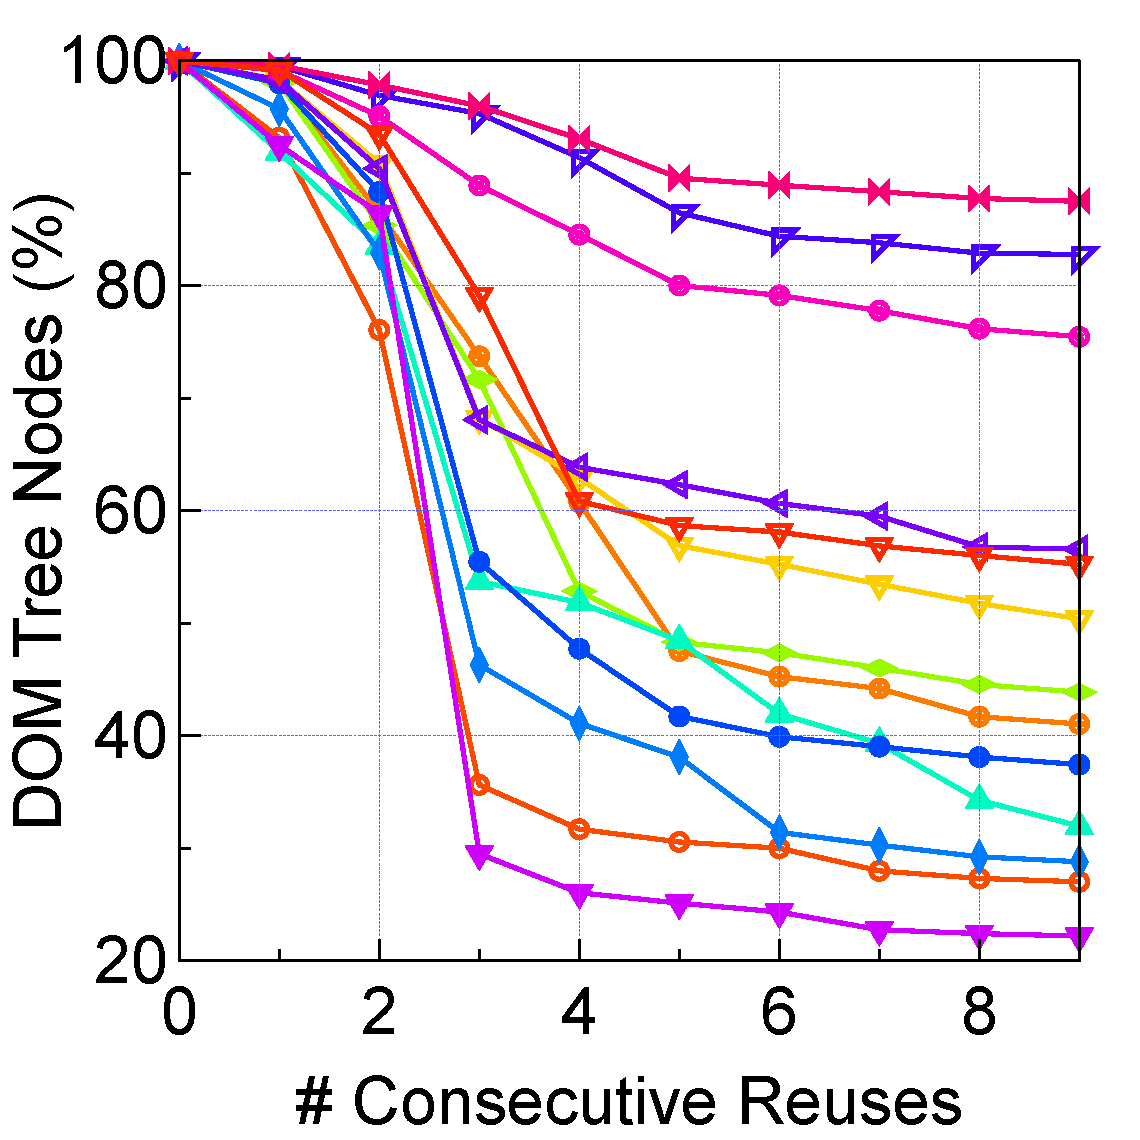
\includegraphics[trim=0 00 0 0, clip, width=\columnwidth]{cdf-con-reuse}
%    \caption{\small{CDF of DOM tree node consecutive reuse. Each line represents a webpage that we study.}}
%    \label{fig:con-reuse}
%  \end{minipage}
%  \hspace*{25pt}
%  \begin{minipage}[b]{0.3\columnwidth}
%    \centering
%    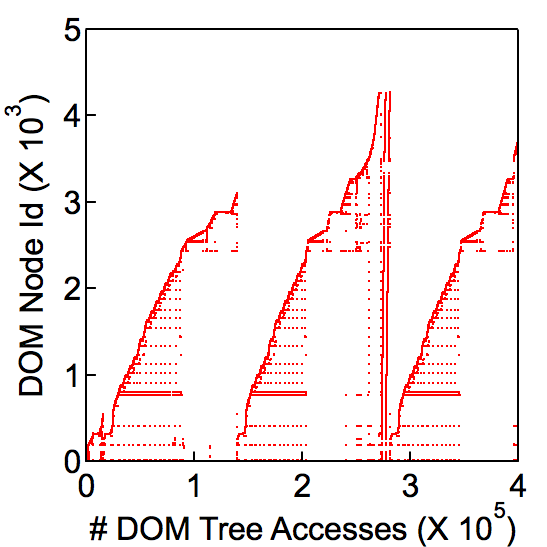
\includegraphics[trim=0 0 0 0, clip, width=\columnwidth]{data-acs.png}
%    \caption{\small{Access pattern of the DOM tree at the granularity of individual DOM tree node.}}
%    \label{fig:data-acs}
%  \end{minipage}
%\end{figure}
%
%Such strong data reuse is due to DOM tree traversals in Web applications.
%To illustrate this,~\Fig{fig:data-acs} shows a representative data
%access patterns to the DOM tree from \website{www.slashdot.org}. Each ($x, y$)
%point is read as follows. The $x$-th access to the DOM tree operated on the
%$y$-th DOM node. We observe a streaming pattern. The browser engine typically
%operates on one DOM tree node heavily and traverses to the next one. Many
%kernels require such traversals. For example, in order to match CSS rules with
%descendant selectors such as~``\textsf{div p},'' which selects any~\textsf{<p>}
%element that is a descendant of~\textsf{<div>} in the DOM tree,
%the~\textit{Style} kernel must traverse the DOM tree, one node at a time, to
%identify the inheritance relation between two nodes.
%
%We propose the DOM cache to capture the DOM tree data locality. It sits between
%the processor and the L1 cache, effectively behaving as an L0 cache. Each cache
%line contains the entire data for one DOM tree node. We implement each cache
%line as a set of independently addressable registers, where each register holds
%one attribute of the DOM tree node, because each node has multiple attributes
%that must be individually accessed.
%
%It is possible to implement the DOM cache entirely in hardware, similar to a
%normal data cache. However, we choose to implement it as a ``software-managed''
%cache--i.e., the data is physically stored in hardware memory, and the software
%performs the actual cache management, such as insertion and replacement. Prior
%work has demonstrated effective software-managed cache
%implementations~\cite{swcache}.
%
%Our motivation for a software-managed cache is to avoid the complexity of a
%hardware cache. Typically, the cache involves hardware circuitry whose overhead
%can be high, especially for extremely small cache sizes. Moreover, we find the software
%overhead is relatively insignificant because of the relative simple cache design.
